\documentclass{article}
\usepackage[utf8]{inputenc}
\usepackage[spanish]{babel}
\usepackage{listings}
\usepackage{graphicx}
\graphicspath{ {images/} }
\usepackage{cite}

\begin{document}

\begin{titlepage}
    \begin{center}
        \vspace*{1cm}
            
        \Huge
        \textbf{Informe de Implementación - Informatica II.}
            
        \vspace{0.5cm}
        \LARGE
            
        \vspace{1.5cm}
            
        \textbf{Luis Miguel Gil Rodriguez.}
        \\
        \textbf{Maverick Sossa Tobon.}
        \vfill
        \vspace{0.8cm}
            
        \Large
        Despartamento de Ingeniería Electrónica y Telecomunicaciones\\
        Universidad de Antioquia\\
        Medellín\\
        Septiembre de 2021
            
    \end{center}
\end{titlepage}
\tableofcontents
\newpage
\section{Sección introductoria} \label{intro}
En este documento, podremos encontrar las ideas para abordar el parcial numero dos del curso Informatica II. Encontraremos en el detalles tales como el lgoritmo de redimensionamiento de imagenes para luego se mostrados en una martriz de LEDs de un tamaño ce 16 por 16 LEDs.

\section{Clases implementadas} \label{clases implementadas}
Se diseña una clase que, a partir de unos datos inciales y unos métodos, cumple el objetivo de redimensionar una imagen al tamaño de una matriz de leds. 
Un archivo de cabecera, en c++, por lo general contiene la definición de los miembros públicos, privados o protegidos de detarminada clase. Son utilidad visual se basa en que proporcionan una idea general de aquello que constituye tal clase. Entonces, para dar ilustración del programa, se desea mostrarlo. 

\begin{lstlisting}[language=C++, label=codigo_matrices_int]


#include <iostream>
#include <QImage>
#include <fstream>

using namespace std;

class ImageResize
{
public:
    // Destructor. Es necesario dada la existencia de ciertos
    // atributos creados en el heap
    ~ImageResize();
    
    // Constructor con parametros. Los necesario para el completo 
    // funcionamiento del programa
    ImageResize(int _wLeds, int _hLeds, string _fileNameImg, 
    string _fileNameTxt);

    // [ SUBMUESTREO ]
    // Submuestreo en donde la division es exacta
    void subDivisionExact();
    // Submuestreo en donde la division no es exacta
    void subNoDivisionExact();

    // [ SOBREMUESTREO ]
    // Analogo a submuestreo
    void sobreDivisionExact();
    void sobreNoDivisionExact();
    
    // A partir de las dimensiones de la matriz de leds
    // y la imagen, determina que metodo, entre los de 
    // submuestreo y sobremuestreo, se debe ejecutar para 
    // la correcta redimension de la imagen
    void categorizeAlgorithm();
    
    // Una vez realizado el proceso de redimension, se 
    // ejecuta para guardar la informacion en un .txt
    void SaveImgTxt();
    
private:

    int mWidthL; // Ancho de matriz de leds
    int mHeightL; // Alto/largo de matriz de leds
    
    // Ruta y nombre de la imagen
    string mFileNameImg; 
    
    // Nombre y ruta del archivo .txt
    string mFileNameTxt;
    
    // Objeto que contiene la informacion de la imagen
    // Se inicializa en el constructor
    QImage *IMG; 

    /// [ MATRICES DE CADA COLOR]
    // Contendran la informacion de la imagen de cada 
    // color. Estan en el heap.
    // Se incializan en el constructor.
    int **mImgRed;
    int **mImgGreen;
    int **mImgBlue;
};

\end{lstlisting}
\section{Esquema de las clases implementadas} \label{esquema}
En la ejecución del programa, hay un flujo ordenado de datos y tareas que permiten cumplir un objetivo: redimensionar una imagen. Notar tal flujo en una representación gráfica significará, realmente, obtener una idea general del funcionamiento del programa.
Por tanto, se hace efectivo la realización de un diagrama ilustrativo. 
\begin{figure}[h]
  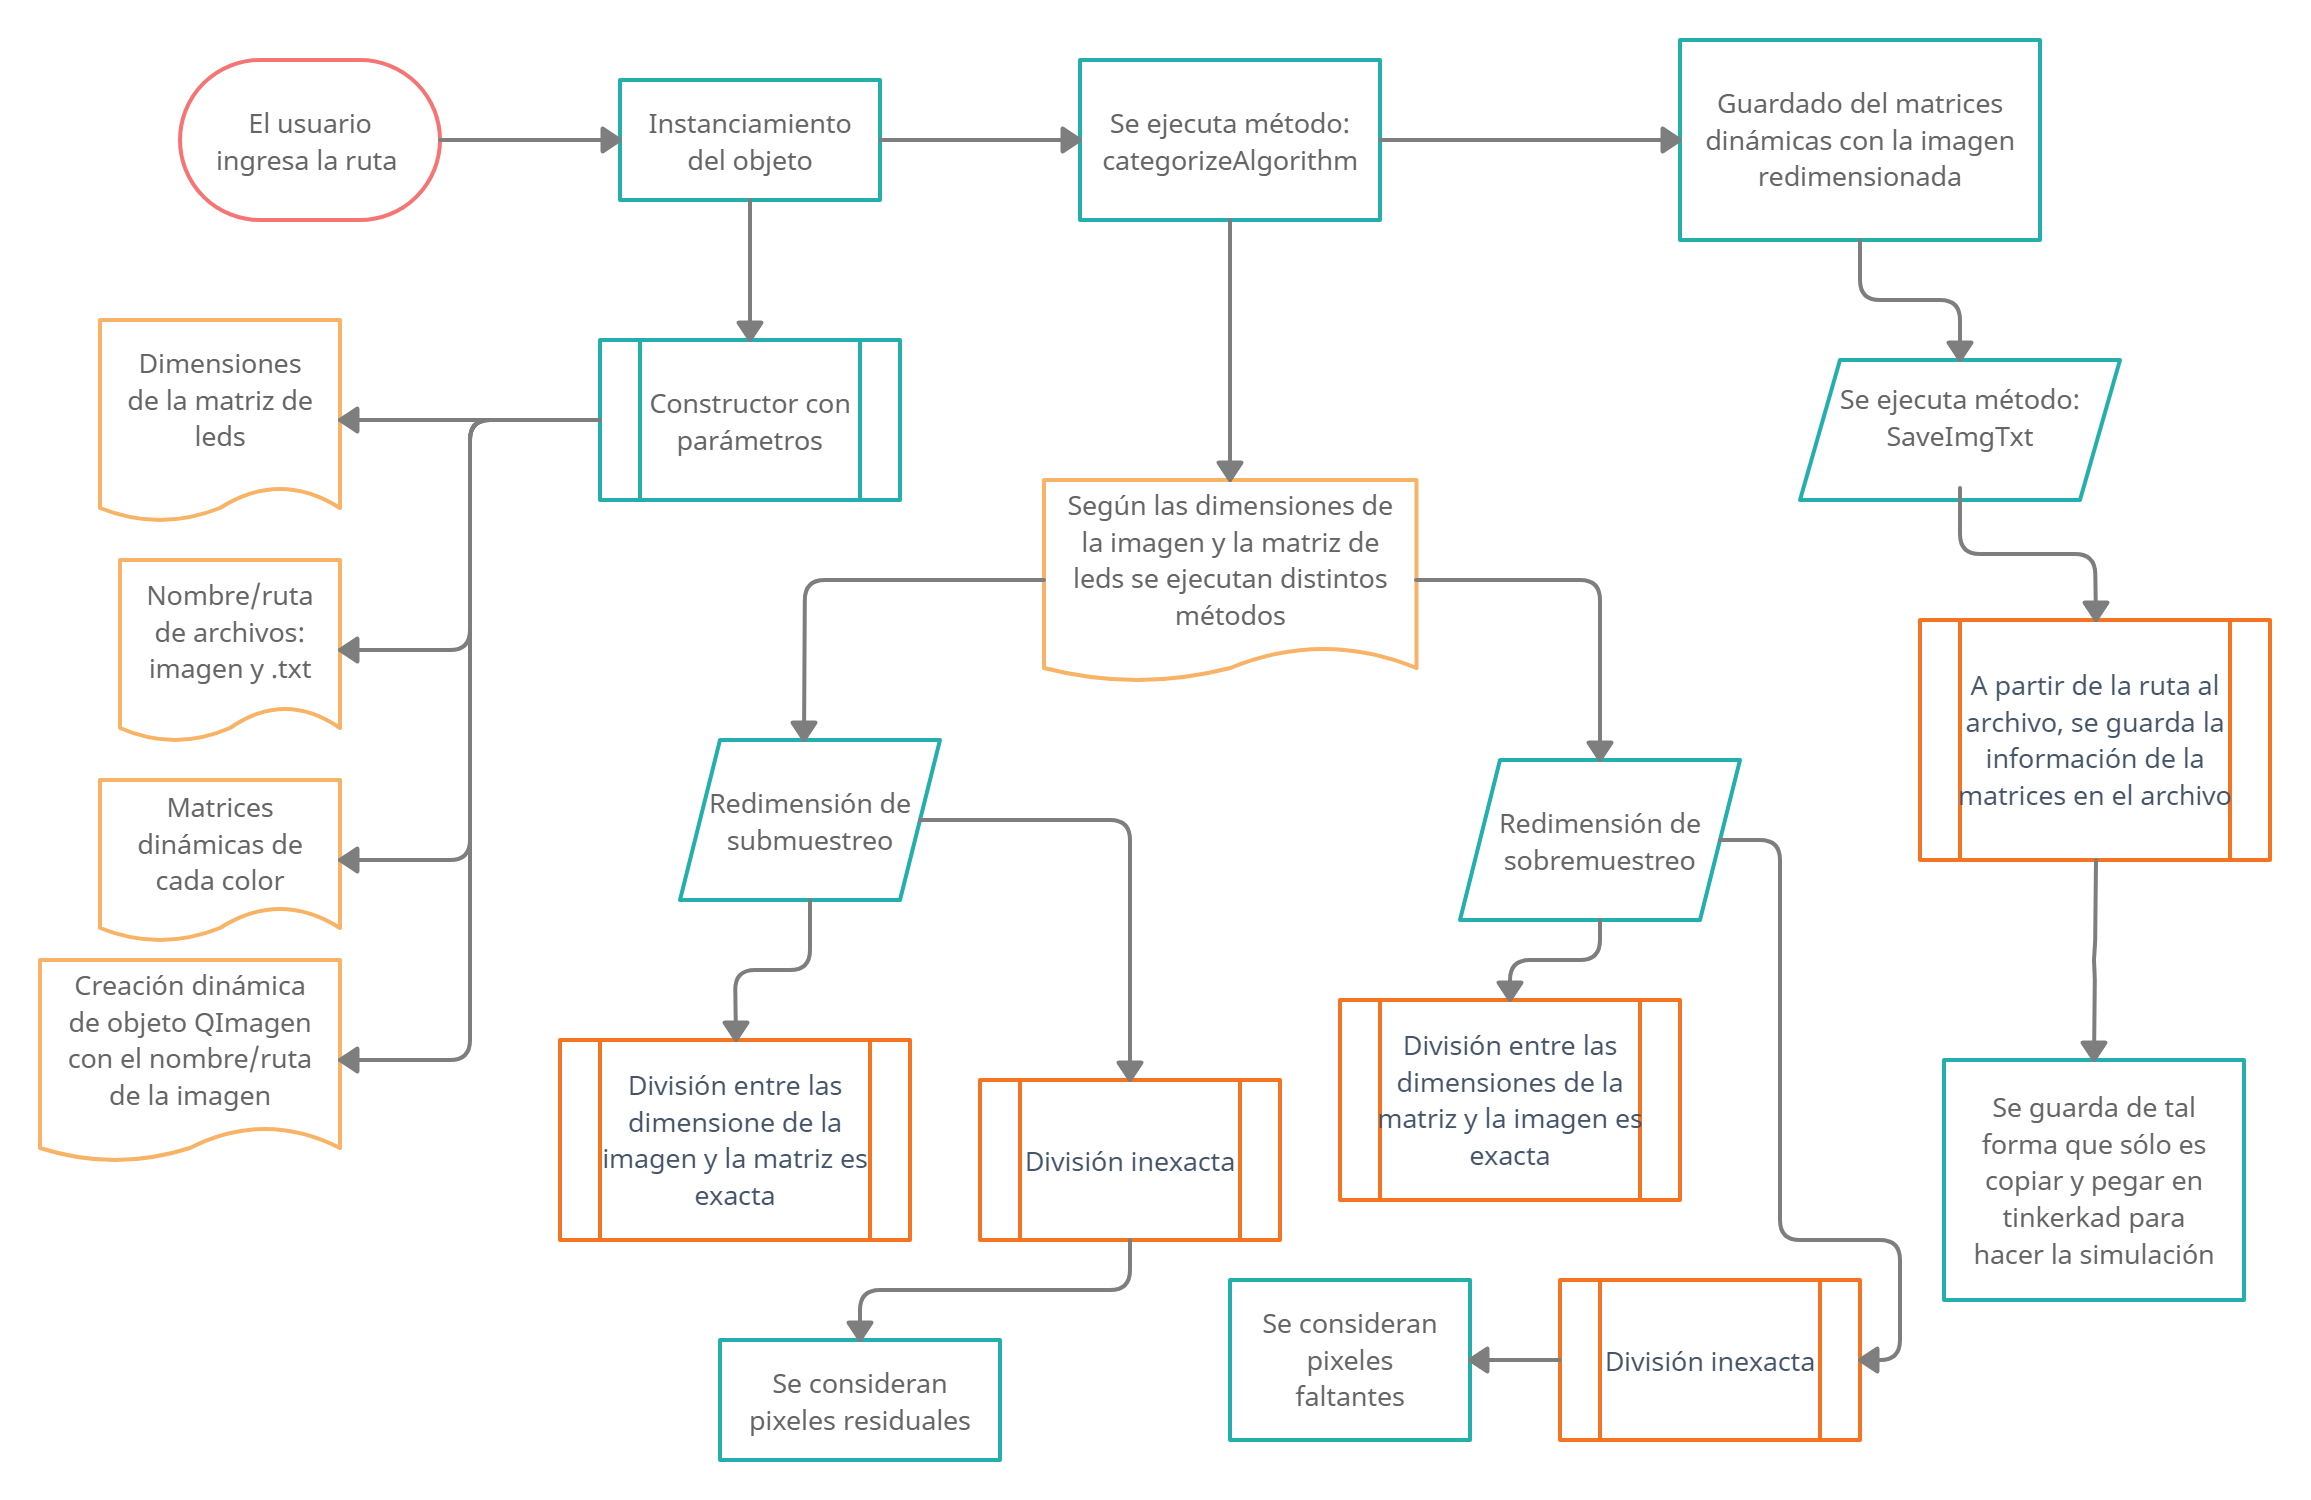
\includegraphics[width=10cm]{Esquema_Parcial_II.png}
  \centering
  \caption{Representación gráfica}
  \label{fig:diagrama_ilustracion}
\end{figure}

\section{Módulos de código implemetado} \label{módulos de código}
Ciertamente el orden es algo a considerar en la programación, y aún más cuando los programas son grandes, de miles y miles de lineas de código. En estos casos resulta práctico usar la programación modular. No solo se dentrá menos cargado un archivo, sino que también, al distribuir efectivamente el código, se podrá tener un acceso y una vista más rápida y cómoda al código por el ordenamiento usado. 



\begin{lstlisting}[language=C++, label=codigo_matrices_int]

/// [ PRIMER MODULO ]

// modulo: imageresize.cpp
// Metodos relacionados directamente con el 
// proceso de redimension de la imagen
#include "imageresize.h"

// Se habla varias veces de "divisionExact". 
// Se refiere a que: en submuestreo, la division entre 
// el tamano de la imagen y el de matriz es o no exacta; 
// y el sobremuestreo se refiere a que la division entre
// el tamano de la matriz y el de la imagen es o no exacta.

/// [ METODOS DE SUBMUESTREO ]

void ImageResize::subDivisionExact()
{
    // Dimensiones de la imagen
    int width = IMG->width();
    int height = IMG->height();
    
    // Tamano del salto en las columas 
    // y en las filas
    int pixelsColum = width/mWidthL;
    int pixelsRow = height/mHeightL;

    for (int i = 0; i < mHeightL ; i++) {
        for (int j = 0; j < mWidthL; j++) {
            // Asignacion de los colores a cada matriz
            // Con saltos sobre la imagen de la forma: 
            // j*pixelsColum; i*pixelsRow
            
        }
    }
}

void ImageResize::subNoDivisionExact()
{
    int width = IMG->width();
    int height = IMG->height();
    // La idea de este caso es el siguiente:
    // Como la division no es exacta, si no se consideran los pixeles
    // restantes se pierde informacion posiblemente importante.
    //  Esta cantidad de pixeles que restan se obtienen con las 
    // variables: pixResColum, pixResRow.
    // Entonces la forma de considerar estos pixeles restantes con
    // que, cada vez que se coje un pixel dando su posicion,
    // sumamos uno a la coordenada x o y, dependiendo del caso.

    int pixelsColum = width/mWidthL;
    int pixelsRow = height/mHeightL;

    // Indicadores de desde donde empezar a considerar los pixeles
    // restantes
    int pixResColum = width % mWidthL;
    int pixResRow = height % mHeightL;

    // Cantidad de pixeles a correr en la filas (row)
    int contPixR = 0; 
    
    // Cantidad de pixeles a correr en las columanas (column)
    int contPixC = 0; 
    
    for (int i = 0; i < mHeightL; i++ ) {
        if ((mHeightL - pixResRow) <= i) {
            ++contPixR;
        }
        for (int j = 0; j < mWidthL; j++) {
            // Caso en que se corren los pixeles en la filas(row) y
            // columnas(Colum) a la vez
            if ((mHeightL - pixResRow) <= i  && (mWidthL 
            - pixResColum) <= j) {
                ++contPixC;
                // Asignacion de los colores a cada matriz
                
            }// Caso en que no se corren ni en la filas(row) y 
            // columnas(Colum)
            else if ((mHeightL - pixResRow) > i  && (mWidthL 
            - pixResColum) > j){
                // Asignacion de los colores a cada matriz
                
            }// Caso en que solo se corren en las fillas(row)
            else if ((mHeightL - pixResRow) <= i) {
                // Asignacion de los colores a cada matriz
                
            }// Caso en solo se corren en las columnas(column)
            else {
                ++contPixC;
                // Asignacion de los colores a cada matriz
            }
        }
        contPixC = 0;
    }

}

/// [ METODOS DE SOBREMUESTREO ]

void ImageResize::sobreDivisionExact()
{
    int width = IMG->width();
    int height = IMG->height();

    int pixelsColum = mWidthL/width;
    int pixelsRow = mHeightL/height;

    int red;
    int green;
    int blue;

    for (int i = 0; i < height; i++) {
        for (int j = 0; j < width; j++) {
            // Se coge el color a replicar
            
            // En la matriz de leds, se pone repetitivamene tal color
            for (int iCopy = 0; iCopy < pixelsRow; iCopy++) {
                for (int jCopy = 0; jCopy < pixelsColum; jCopy++) {
                    // Asignacion de los colores a cada matriz
                }
            }
        }
    }
}

void ImageResize::sobreNoDivisionExact()
{
    int width = IMG->width();
    int height = IMG->height();

    // Indican la cantidad de veces a replicar un pixel, ya sea de
    // columna o fila
    int pixelsColum = mWidthL/width;
    int pixelsRow = mHeightL/height;

    // Indican la cantidad de pixels faltantes para completar la 
    // matriz de leds
    int pixResColum = mWidthL % width;
    int pixResRow = mHeightL % height;

    // Contadores auxuliares para el relleno de pixeles en 
    // filas y columnas
    // Se inicializan en -1 porque en caso contrario
    // indexan la matriz en posiciones invlidas
    int contPixR = -1;
    int contPixC = -1;

    int red;
    int green;
    int blue;

    for (int i = 0; i < height; i++) {
        if ((height - pixResRow) <= i) {
            contPixR++;
        }

        for (int j = 0; j < width; j++) {
            red = IMG->pixelColor(j, i).red();
            green = IMG->pixelColor(j, i).green();
            blue = IMG->pixelColor(j, i).blue();

            // Caso en que rellenan con pixeles en la
            // filas(row) y las columnas(colum)
            if ((height - pixResRow) <= i  && (width - 
            pixResColum) <= j) {
                contPixC++;
                for (int iCopy = 0; iCopy < pixelsRow + 1; iCopy++) {
                    for (int jCopy = 0; jCopy < pixelsColum + 1;
                     jCopy++) {
                        // Asignacion de los colores a cada matriz
                    }
                }
            }// Caso en que no se rellenan con 
            // pixeles ni en las filas(row) ni en 
            // las columnas(colum)
            else if ((height - pixResRow) > i && (width 
            - pixResColum) > j) {
                for (int iCopy = 0; iCopy < pixelsRow; iCopy++) {
                    for (int jCopy = 0; jCopy < pixelsColum; 
                    jCopy++) {
                        // Asignacion de los colores a cada matriz
                    }
                }
            }// Caso en que se rellenan con pixeles 
            // solo en las filas(row)
            else if ((height - pixResRow) <= i) {
                for (int iCopy = 0; iCopy < pixelsRow + 1; iCopy++) {
                    for (int jCopy = 0; jCopy < pixelsColum; 
                    jCopy++) {
                        // Asignacion de los colores a cada matriz
                    }
                }
            }// Caso en que se rellenan con pixeles 
            // solo en las columnas(colum)
            else {
                contPixC++;
                for (int iCopy = 0; iCopy < pixelsRow; iCopy++) {
                    for (int jCopy = 0; jCopy < pixelsColum + 1;
                     jCopy++) {
                        // Asignacion de los colores a cada matriz
                    }
                }
            }
        }contPixC = -1;
    }
}

/// [ SEGUNDO MODULO ]

// modulo: img_rsz_functs.cpp
// Metodos que no estan realacionados directamente  
// con el proceso de redimension de la imagen
#include "imageresize.h"

#include "imageresize.h"

/// [ FUNCIONES QUE NO INCLUYEN REDIMENSIONAMIENTO ]


void ImageResize::categorizeAlgorithm()
{
    int width = IMG->width();
    int height = IMG->height();

//    float categW = width / mWidthL;
//    float categH = height / mHeightL;

    if ((width >= mWidthL) && (height >= mHeightL)) {
        // En este caso se realiza submuestreo
        // Ejecucion metodos de submuestreo
        
    }else if ((width <= mWidthL) && (height <= mWidthL)) {
        // En este se hace sobremuestreo
        // Ejecucion metodos de sobremuestreo
        
    }else if ((width >= mWidthL) && (height <= mHeightL)) {
        // En este caso se hace submuestreo sobre el ancho,
        // y sobremuestreo sobre el alto
        
    }else if((width <= mWidthL) && (height >= mHeightL)) {
        // En este caso de hace sobremuestreo sobre el ancho,
        // y submuestreo sobre el alto
    }
}


ImageResize::ImageResize(int _wLeds, int _hLeds, 
string _fileNameImg, string _fileNameTxt)
{
    // [ Inicializacion atributos basicos ]

    mWidthL = _wLeds;
    mHeightL = _hLeds;
    mFileNameImg = _fileNameImg;
    mFileNameTxt = _fileNameTxt;

    IMG = new QImage(mFileNameImg.c_str());

    // [ Inicializacion dinamica de matrices que contendran 
    // los datos de la img redimensionada ]

    mImgRed = new int *[mHeightL];
    mImgGreen = new int *[mHeightL];
    mImgBlue = new int *[mHeightL];
    for (int i = 0; i < mHeightL; i++) {
        mImgRed[i] = new int [mWidthL];
        mImgGreen[i] = new int [mWidthL];
        mImgBlue[i] = new int [mWidthL];
    }
}

void ImageResize::SaveImgTxt()
{
    // El metodo realiza el proceso de guardado de 
    // la imagen redimensionda en un archivo txt

    ofstream archImg(mFileNameTxt);

    if (!archImg.is_open()) {
        cout << "Error al abrir archivo" << endl;
        exit(1);
    }

    // [ Se almacena el color Red ]
    archImg << "uint8_t RedMatrix [256] = { \n";
    
    for (int i = 0; i < mHeightL; i++) {

        for (int j = 0; j < mWidthL; j++) {
            // Se considera el 255 por el error de tinkerkad
            // Se guarda en el archivo el dato de la
            // matriz de la posicion ij
        }
        archImg << "\n";
    }
    archImg << "}; \n\n";

    // [ Se almacena el color Green ]
    archImg << "uint8_t GreenMatrix [256] = { \n";
    for (int i = 0; i < mHeightL; i++) {

        for (int j = 0; j < mWidthL; j++) {
            // Se considera el 255 por el error de tinkerkad
            // Se guarda en el archivo el dato de la
            // matriz de la posicion ij
        }
        archImg << "\n";
    }
    archImg << "}; \n\n";

    // [ Se almacena el color Blue ]
    archImg << "uint8_t BlueMatrix [256] = { \n";
    for (int i = 0; i < mHeightL; i++) {

        for (int j = 0; j < mWidthL; j++) {
            // Se considera el 255 por el error de tinkerkad
            // Se guarda en el archivo el dato de la
            // matriz de la posicion ij
        }
        archImg << "\n";
    }
    archImg << "}; \n\n";

    archImg.close();

}

ImageResize::~ImageResize()
{
    // Destructor que elimina los arreglos dinamicos de la imagen

    for (int i = 0; i < mHeightL; i++) {
        delete [] mImgRed[i];
        delete [] mImgGreen[i];
        delete [] mImgBlue[i];
    }
    delete [] mImgRed;
    delete [] mImgGreen;
    delete [] mImgBlue;


}

    
\end{lstlisting}


\section{Circuito.} \label{circuito}
Para la implementación del circuito en la plataforma Tinkercad, primeramente se comenzaron a realizar ensayos con una tira de 16 Neopixeles, la cual se conecta de la siguiente manera:
\begin{enumerate}
  \item La primera fila se conecta al puerto 2 del Arduino.
  \item Se le suministra potencia de 5 Voltios a la tira de Neopixel procedentes del Arduino.
  \item Se conecta el polo a tierra procedente del Arduino a la tira del Neopixel.
\end{enumerate}
\begin{figure}[h]
  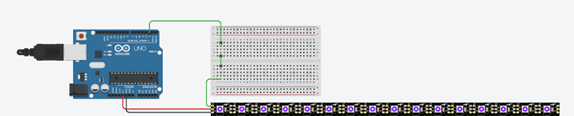
\includegraphics[width=10cm]{figura_1.png}
  \centering
  \caption{Prender fila numero uno de la matriz.}
  \label{fig:fila_uno}
\end{figure}
Se comenzó la etapa de pruebas con la tira de Neopixel, ejemplo de algunas pruebas que se realizaron:
\begin{enumerate}
    \item Cómo prender un Neopixel en específico.
    \item Cómo mostrar un patrón en una tira (ejemplo: Solo prender las posiciones impares, solo prender las posiciones pares).
    \item Cómo prender todos los leds e a la vez.
\end{enumerate}
Una vez superada esta etapa de prueba se agregaron las 15 filas restantes, para obtener una especie de matriz de 16 X 16, en primer lugar se realiza la conexión desde la fila uno hasta la fila cinco de la siguiente manera:
\begin{enumerate}
    \item Se conecta entrada de la fila N con la entrada de la fila N+1.
    \item Se conecta la potencia de la fila N con la potencia de la fila N+1.
    \item Se conecta la tierra de la fila N con la tierra de la fila N+1.
\end{enumerate}
Al intentar interactuar con la matriz, por ejemplo prender una Neopixel en específico se evidencio que tenía un comportamiento de prender por columnas, conducta para nada esperada.\\
\begin{figure}[h]
  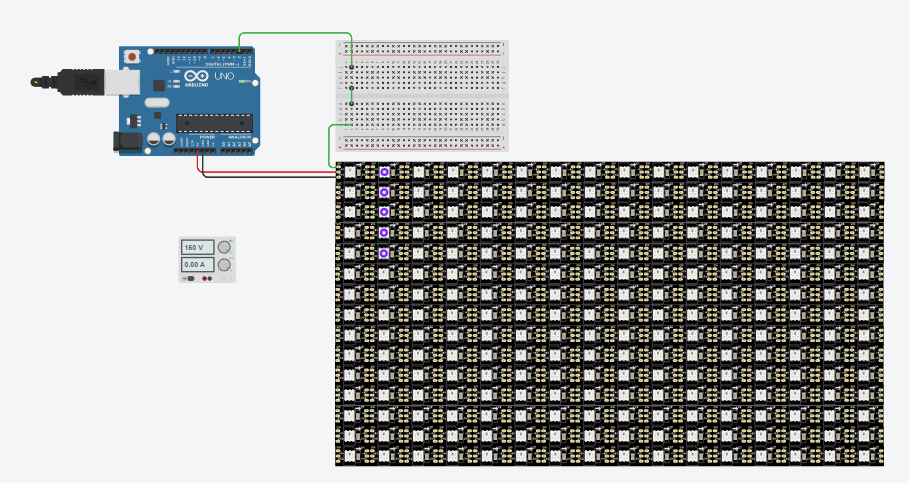
\includegraphics[width=10cm]{figura_2.png}
  \centering
  \caption{Comportamiento no esperado.}
  \label{fig:por_columnas}
\end{figure}
Al evidenciar este comportamiento, de inmediato se repiensa la manera de como realizar satisfactoriamente la conexión. Hasta que se llego hasta la siguiente idea:
\begin{enumerate}
    \item Se conecta salida de la fila N con la entrada de la fila N+1.
    \item Se conecta la potencia de la fila N con la potencia de la fila N+1.
    \item Se conecta la tierra de la fila N con la tierra de la fila N+1.
\end{enumerate}
Luego de haber realizado dicha conexión, se comenzó una nueva etapa de pruebas con el mismo, se intento prender todas las filas conectas, un Neopixel en específico y por último un patrón sencillo, como prender solo las posiciones impares, la diagonal principal de la matriz entre otras pruebas.

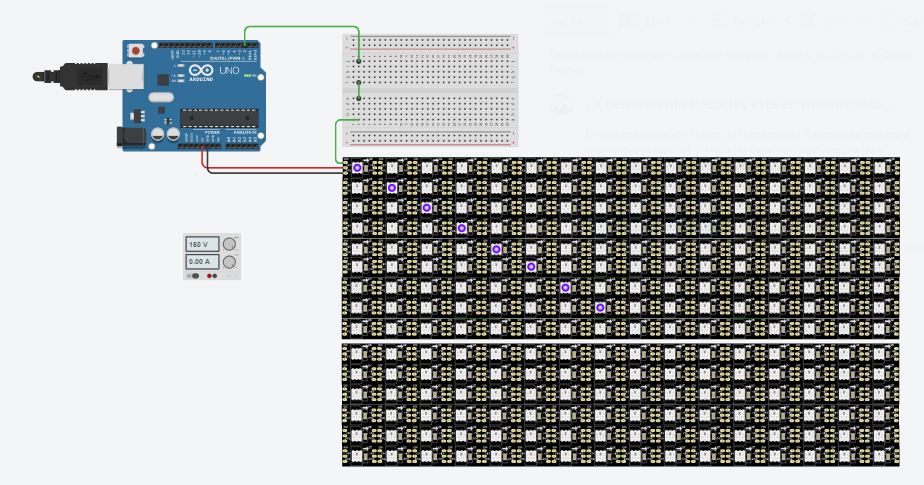
\includegraphics[width=8cm]{figura_3.png}
  
A continuacion se mostrara el circuito desarrollado, cabe mencionar, que el aspecto que aqui se muestra no sera el definiticvo, pues se reorganizaran las tiras de Neopixel de una manera mas estetica.

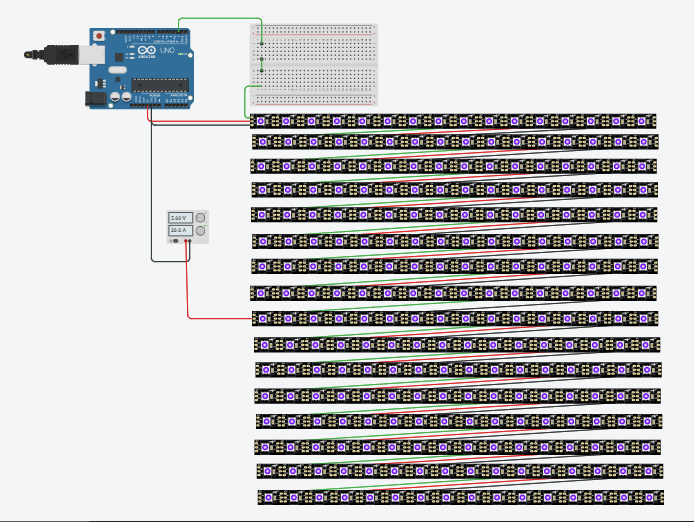
\includegraphics[width=8cm]{figura_4.png}

\begin{enumerate}
    \item Los cables de color verde se encargan de llevar los datos a la matriz de LEDs
    \item Los cables de color Negro representan el Polo a Tierra.
    \item Los cables de color Rojo representan la potencia (5.0 V).
    \item Se conecta un suministro de energia, el cual alimentara la matriz de LEDs, es decir suministrara potencia a partir de la fila 9 de nuestra matriz. Este mismo alimentará con 5.0 Voltios a la matriz de LEDs.
\end{enumerate}
\section{Problemas presentados en la implementacion.} \label{problemas}
\subsection{Con respecto al Circuito.}
Realmente, se tuvo mucho menos inconvenientes en el montaje de este circuito a comparación del Parcial pasado, hemos evidenciado que hemos crecido potencialmente en este ámbito.
El único problema que se tuvo, y ya se mencionó, fue el haber realizado la conexión de la siguiente manera: 
\begin{enumerate}
    \item Se conecta entrada de la fila N con la entrada de la fila N+1.
    \item Se conecta la potencia de la fila N con la potencia de la fila N+1.
    \item Se conecta la tierra de la fila N con la tierra de la fila N+1.
\end{enumerate}
Al momento de realizar pruebas con el circuito nos dimos cuenta de esto por ende, mas temprano que tarde se llegó a una solución definitiva, que fue realizar la conexión de la siguiente manera:
\begin{enumerate}
    \item Conectar salida de la fila N con la entrada de la fila N+1.
    \item Se conecta la potencia de la fila N con la potencia de la fila N+1.
    \item Se conecta la tierra de la fila N con la tierra de la fila N+1.
\end{enumerate}
Después de esto, no se volvió a tener mas inconvenientes en el proceso de montado del circuito.


\subsection{Con respecto al código de Tinkercad.}

Desde que se comenzó a montar el circuito, se viene realizando pruebas con la conexión, todas las pruebas fueron satisfactorias, se realizaron pruebas tales como:
\begin{enumerate}
    \item Prender toda la matriz.
    \item Prender las filas impares.
    \item Prender las filas pares.
    \item Prender la diagonal principal de la matriz.
\end{enumerate}
La única prueba que fallo fue al momento de pasarle la intensidad de cada color RGB por medio de:
\begin{enumerate}
    \item Matriz unidimensional.
    \item Matriz bidimensional.
\end{enumerate}
Mostraremos un ejemplo de como se estaban creando las matrices de la intensidad del color Rojo, tanto bidimensional como unidimensionalmente:
\begin{lstlisting}[language=C++, label=codigo_matrices_int]
int RedMatrix2D [16][16]= {
  {20,20,20,20,20,20,20,20,20,20,20,20,20,20,20,20},
  {20,20,20,20,20,20,20,20,20,20,20,20,20,20,20,20},
  {20,20,20,20,20,20,20,20,20,20,20,20,20,20,20,20},
  {20,20,20,20,20,20,20,20,20,20,20,20,20,20,20,20},
  {20,20,20,20,20,20,20,20,20,20,20,20,20,20,20,20},
  {20,20,20,20,20,20,20,20,20,20,20,20,20,20,20,20},
  {20,20,20,20,20,20,20,20,20,20,20,20,20,20,20,20},
  {20,20,20,20,20,20,20,20,20,20,20,20,20,20,20,20},
  {20,20,20,20,20,20,20,20,20,20,20,20,20,20,20,20},
  {20,20,20,20,20,20,20,20,20,20,20,20,20,20,20,20},
  {20,20,20,20,20,20,20,20,20,20,20,20,20,20,20,20},
  {20,20,20,20,20,20,20,20,20,20,20,20,20,20,20,20},
  {20,20,20,20,20,20,20,20,20,20,20,20,20,20,20,20},
  {20,20,20,20,20,20,20,20,20,20,20,20,20,20,20,20},
  {20,20,20,20,20,20,20,20,20,20,20,20,20,20,20,20},
  {20,20,20,20,20,20,20,20,20,20,20,20,20,20,20,20}
};
int RedMatrix [256]= {
  20,20,20,20,20,20,20,20,20,20,20,20,20,20,20,20,
  20,20,20,20,20,20,20,20,20,20,20,20,20,20,20,20,
  20,20,20,20,20,20,20,20,20,20,20,20,20,20,20,20,
  20,20,20,20,20,20,20,20,20,20,20,20,20,20,20,20,
  20,20,20,20,20,20,20,20,20,20,20,20,20,20,20,20,
  20,20,20,20,20,20,20,20,20,20,20,20,20,20,20,20,
  20,20,20,20,20,20,20,20,20,20,20,20,20,20,20,20,
  20,20,20,20,20,20,20,20,20,20,20,20,20,20,20,20,
  20,20,20,20,20,20,20,20,20,20,20,20,20,20,20,20,
  20,20,20,20,20,20,20,20,20,20,20,20,20,20,20,20,
  20,20,20,20,20,20,20,20,20,20,20,20,20,20,20,20,
  20,20,20,20,20,20,20,20,20,20,20,20,20,20,20,20,
  20,20,20,20,20,20,20,20,20,20,20,20,20,20,20,20,
  20,20,20,20,20,20,20,20,20,20,20,20,20,20,20,20,
  20,20,20,20,20,20,20,20,20,20,20,20,20,20,20,20,
  20,20,20,20,20,20,20,20,20,20,20,20,20,20,20,20
};
\end{lstlisting}
Al iniciar simulación con estas matrices de tipo entero, se evidencio que todo funcionaba perfectamente hasta la hora de que llegaba a la siguiente instrucción:
\begin{lstlisting}[language=C++, label=show]
Leds.show();
\end{lstlisting}
Alli, la matriz no prendia, por ende se comenzó a investigar acerca de la función setPixelColor() de la librería de Neopixel, y nos dimos cuenta que los paramentos de intensidad de cada color (RGB) debía ser del tipo de dato uint8-t, por ende, se cambia el tipo de dato de las matrices de int a uint8-t y funciona correctamente.
Las matrices quedan de la siguiente manera:
\begin{lstlisting}[language=C++, label=codigo_matrices_uint]
uint8_t RedMatrix2D [16][16]= {
  {20,20,20,20,20,20,20,20,20,20,20,20,20,20,20,20},
  {20,20,20,20,20,20,20,20,20,20,20,20,20,20,20,20},
  {20,20,20,20,20,20,20,20,20,20,20,20,20,20,20,20},
  {20,20,20,20,20,20,20,20,20,20,20,20,20,20,20,20},
  {20,20,20,20,20,20,20,20,20,20,20,20,20,20,20,20},
  {20,20,20,20,20,20,20,20,20,20,20,20,20,20,20,20},
  {20,20,20,20,20,20,20,20,20,20,20,20,20,20,20,20},
  {20,20,20,20,20,20,20,20,20,20,20,20,20,20,20,20},
  {20,20,20,20,20,20,20,20,20,20,20,20,20,20,20,20},
  {20,20,20,20,20,20,20,20,20,20,20,20,20,20,20,20},
  {20,20,20,20,20,20,20,20,20,20,20,20,20,20,20,20},
  {20,20,20,20,20,20,20,20,20,20,20,20,20,20,20,20},
  {20,20,20,20,20,20,20,20,20,20,20,20,20,20,20,20},
  {20,20,20,20,20,20,20,20,20,20,20,20,20,20,20,20},
  {20,20,20,20,20,20,20,20,20,20,20,20,20,20,20,20},
  {20,20,20,20,20,20,20,20,20,20,20,20,20,20,20,20}
};
uint8_t RedMatrix [256]= {
  20,20,20,20,20,20,20,20,20,20,20,20,20,20,20,20,
  20,20,20,20,20,20,20,20,20,20,20,20,20,20,20,20,
  20,20,20,20,20,20,20,20,20,20,20,20,20,20,20,20,
  20,20,20,20,20,20,20,20,20,20,20,20,20,20,20,20,
  20,20,20,20,20,20,20,20,20,20,20,20,20,20,20,20,
  20,20,20,20,20,20,20,20,20,20,20,20,20,20,20,20,
  20,20,20,20,20,20,20,20,20,20,20,20,20,20,20,20,
  20,20,20,20,20,20,20,20,20,20,20,20,20,20,20,20,
  20,20,20,20,20,20,20,20,20,20,20,20,20,20,20,20,
  20,20,20,20,20,20,20,20,20,20,20,20,20,20,20,20,
  20,20,20,20,20,20,20,20,20,20,20,20,20,20,20,20,
  20,20,20,20,20,20,20,20,20,20,20,20,20,20,20,20,
  20,20,20,20,20,20,20,20,20,20,20,20,20,20,20,20,
  20,20,20,20,20,20,20,20,20,20,20,20,20,20,20,20,
  20,20,20,20,20,20,20,20,20,20,20,20,20,20,20,20,
  20,20,20,20,20,20,20,20,20,20,20,20,20,20,20,20
};
\end{lstlisting}
\subsection{Con respecto a Qt.}
El primer problema con el que nos encontramos a la hora de la implementación, lo evidenciamos al momento de aplicarle el algoritmo de submuestreo a la siguiente imagen:
\begin{figure}[h]
  
\includegraphics[width=10cm]{bandera_con_problemas.jpg}
  \centering
  \caption{Bandera que presentaba problemas.}
  \label{fig:guia}
\end{figure}
Resulta que la imagen tiene varios pixeles con las siguientes intensidades de color:
\begin{enumerate}
    \item Red = 255
    \item Green = 255
    \item Blue = 255
\end{enumerate}
Y al intentarlo mostrar en la matriz de LEDs tenia un comportamiento bastante extraño, por lo que se recordó lo dicho en la asignación del parcial y redujimos en 1 unidad cada intensidad si resultaba ser [255,255,255]
Luego de aplicar dicho cambio al algoritmo, se pudo mostrar de forma satisfactoria la imagen:
\begin{figure}[h]
  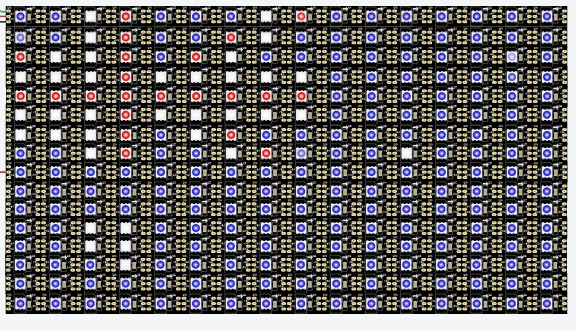
\includegraphics[width=10cm]{bandera_en_matriz.jpeg}
  \centering
  \caption{Bandera en la matriz.}
  \label{fig:guia}
\end{figure}

\subsection{Con respecto a Git y Github.}
Nos vimos fuertemente afectados en cuanto a la coordinación en el repositorio, pues el realizar las cosas en un orden poco adecuado o utilizando comandos incorrectos, trajo como consecuencia que no se pudieran hacer commits, o se realizara un merge “raro” entre una rama y otra.
\\
\\
Después de una ayuda del profesor Jonathan, se esclarecen los problemas y se crea una guía para que esto no nos vuelva a suceder.
\begin{figure}[h]
  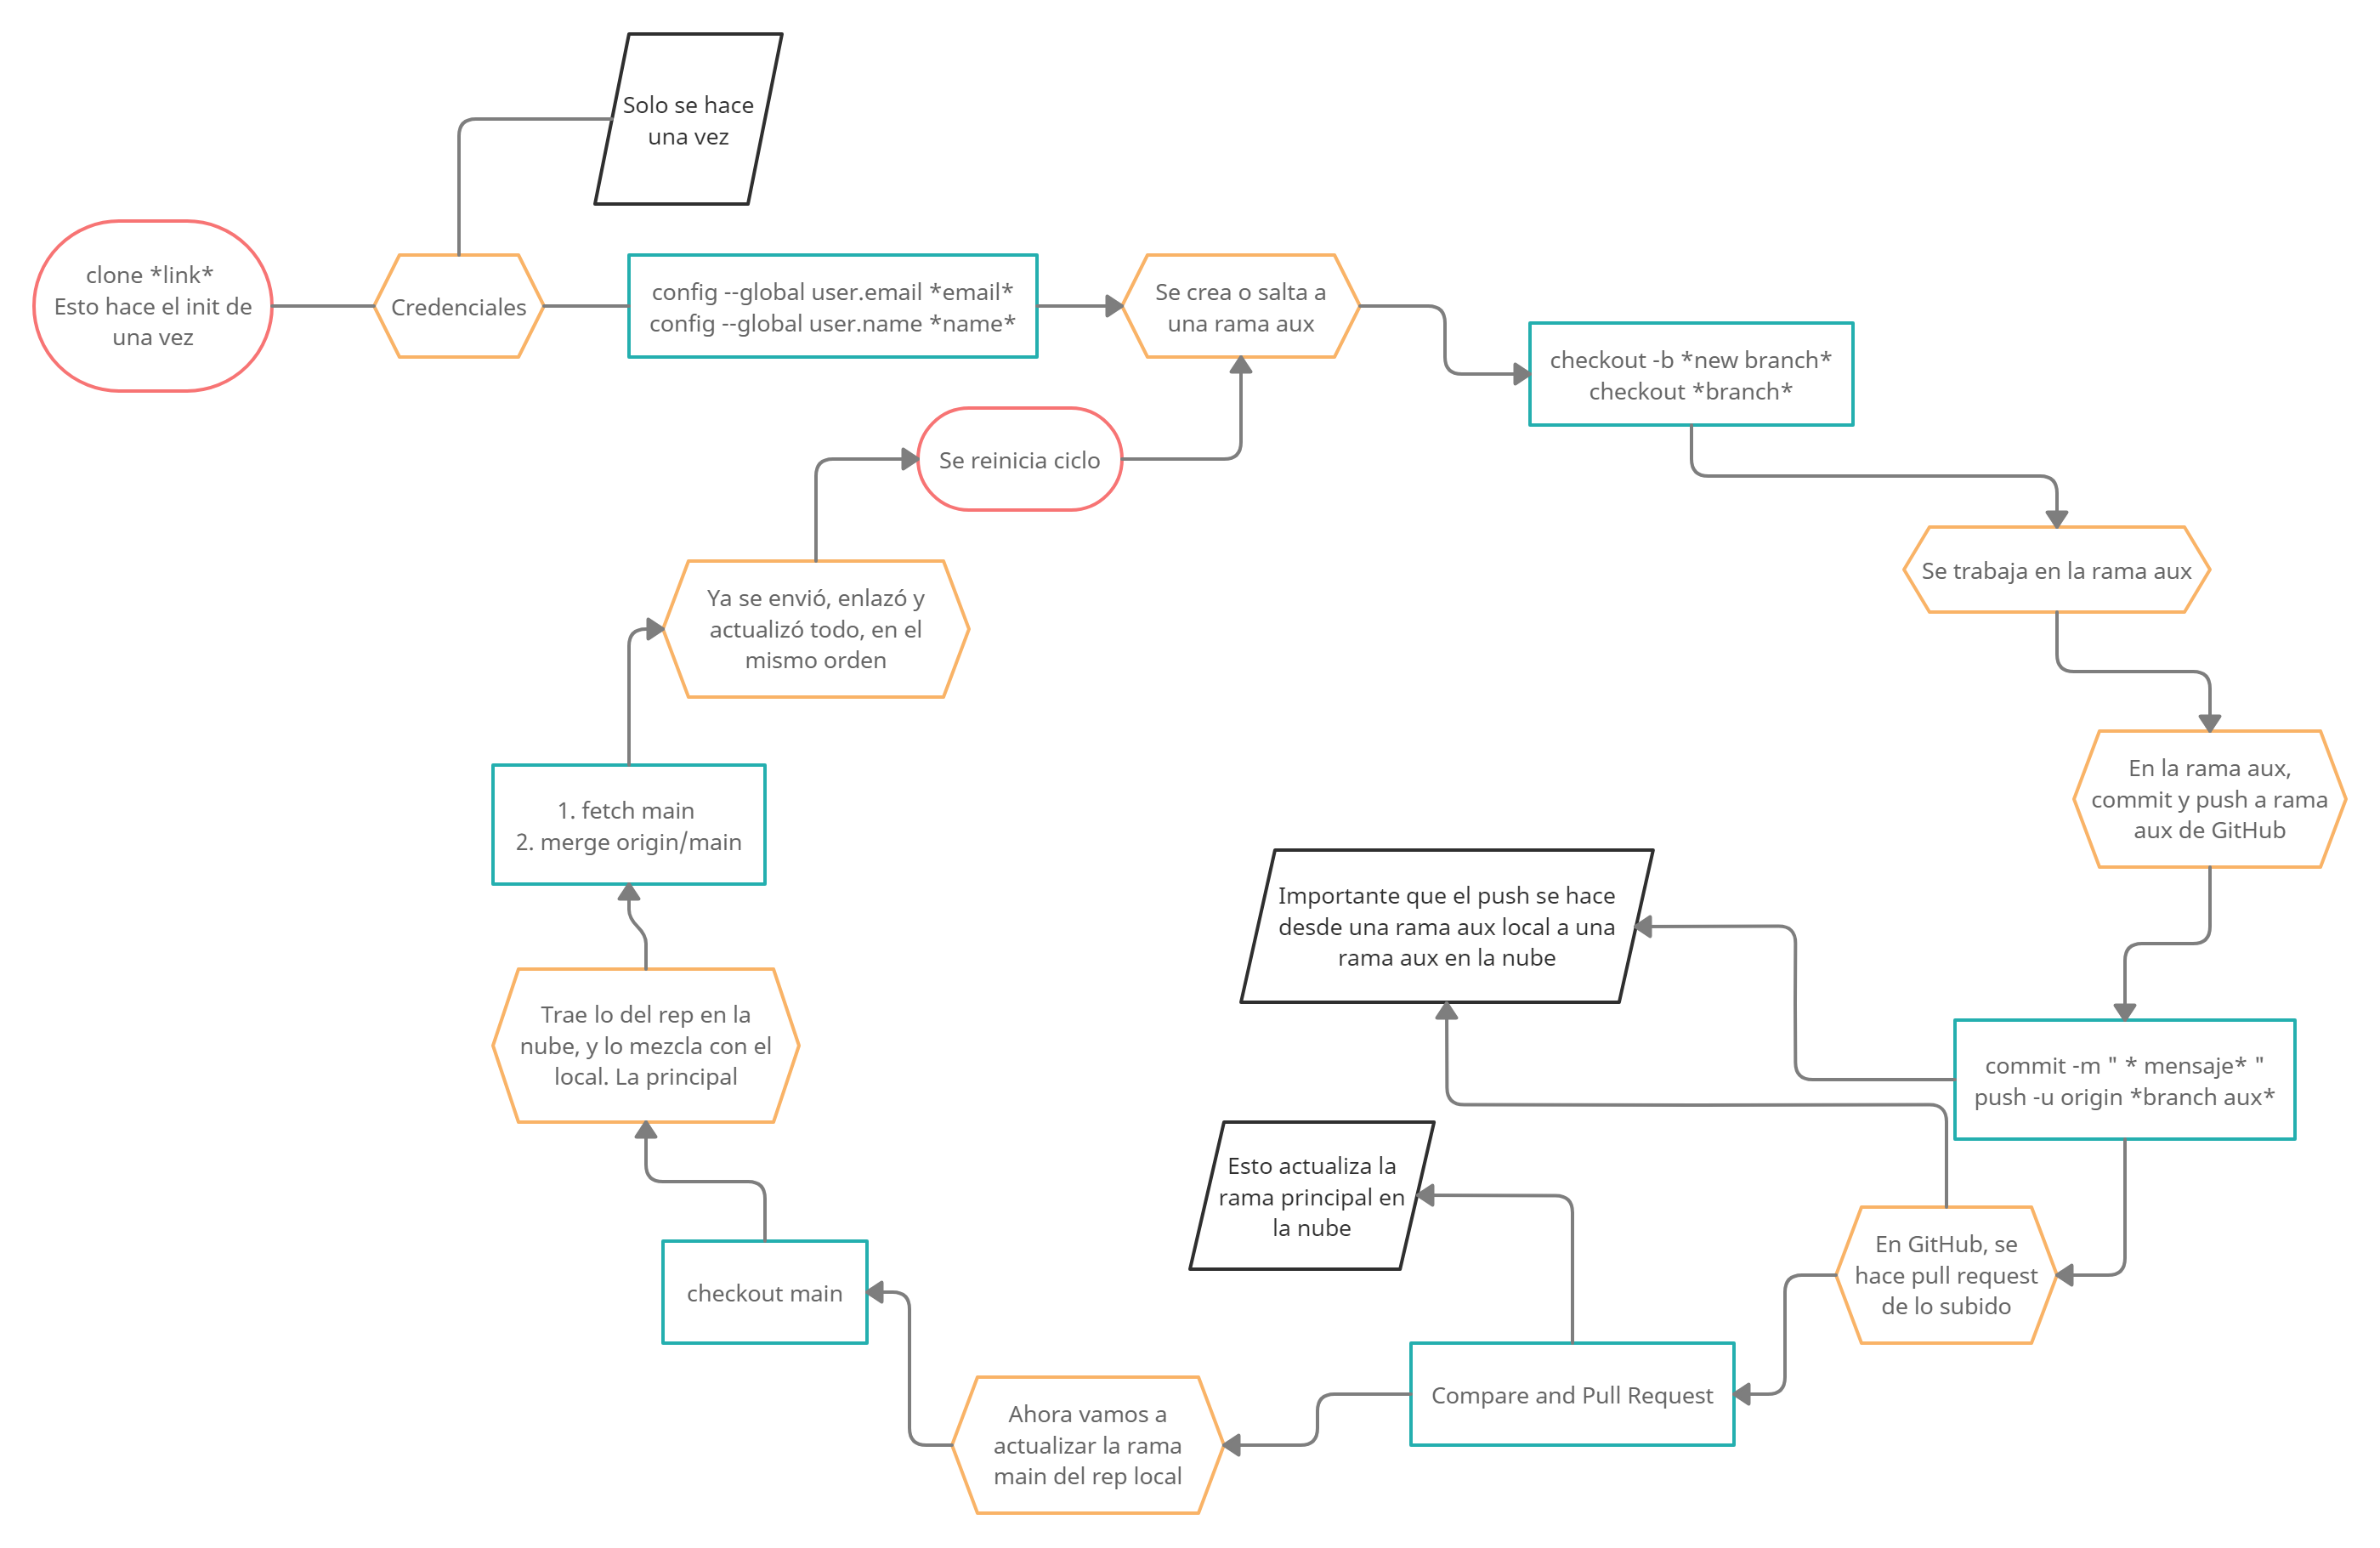
\includegraphics[width=10cm]{Guia_GitHub_GitBash.jpg}
  \centering
  \caption{Diagrama de flujo guia GitBash.}
  \label{fig:guia}
\end{figure}
\bibliographystyle{IEEEtran}
\bibliography{references}
\end{document}
